\section{Python Overview}
\begin{itemize}
    \item \textbf{Origins:} Developed by Guido van Rossum with a focus on simplicity and power.
    \item \textbf{Standard Library:} Known for the "batteries included" philosophy, meaning it comes with an extensive built-in library.
    \item \textbf{Ecosystem:} For engineering tasks, Python replaces Matlab toolboxes with specialized packages like \textbf{NumPy} (numerical data), \textbf{pandas} (data processing), and \textbf{matplotlib} (visualization).
\end{itemize}

\section{Variables and Objects}
In Python, everything is an object. Variables are not containers but \textbf{references} (pointers) bound to objects.

\begin{minipage}{0.4\columnwidth}
    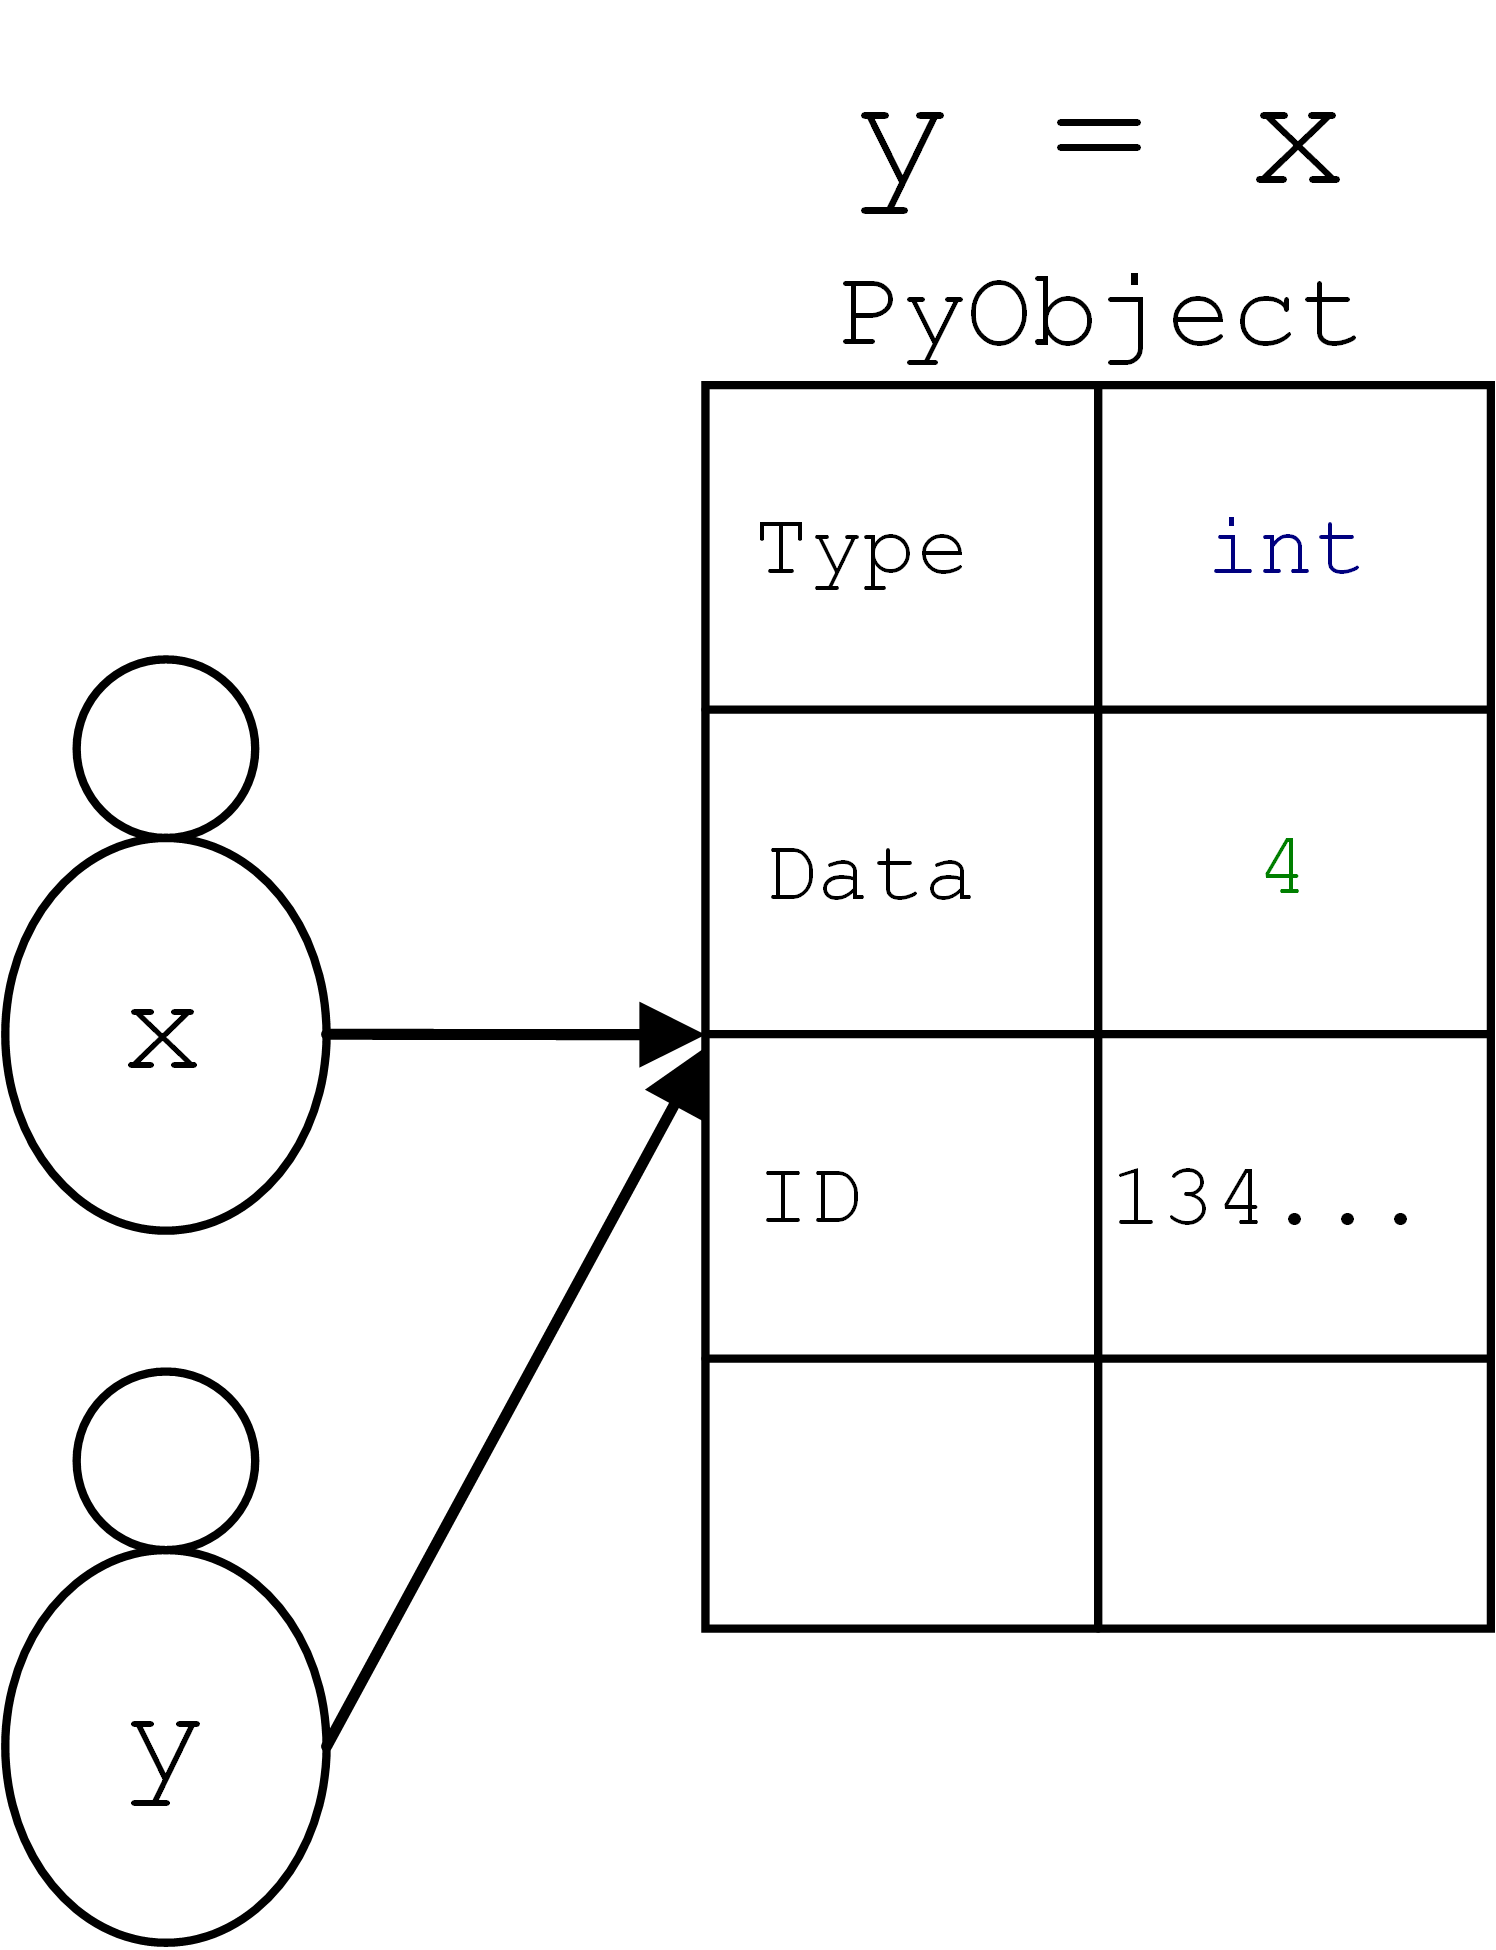
\includegraphics[width=\linewidth]{images/var_2.png}
\end{minipage}\hfil
\begin{minipage}{0.4\columnwidth}
    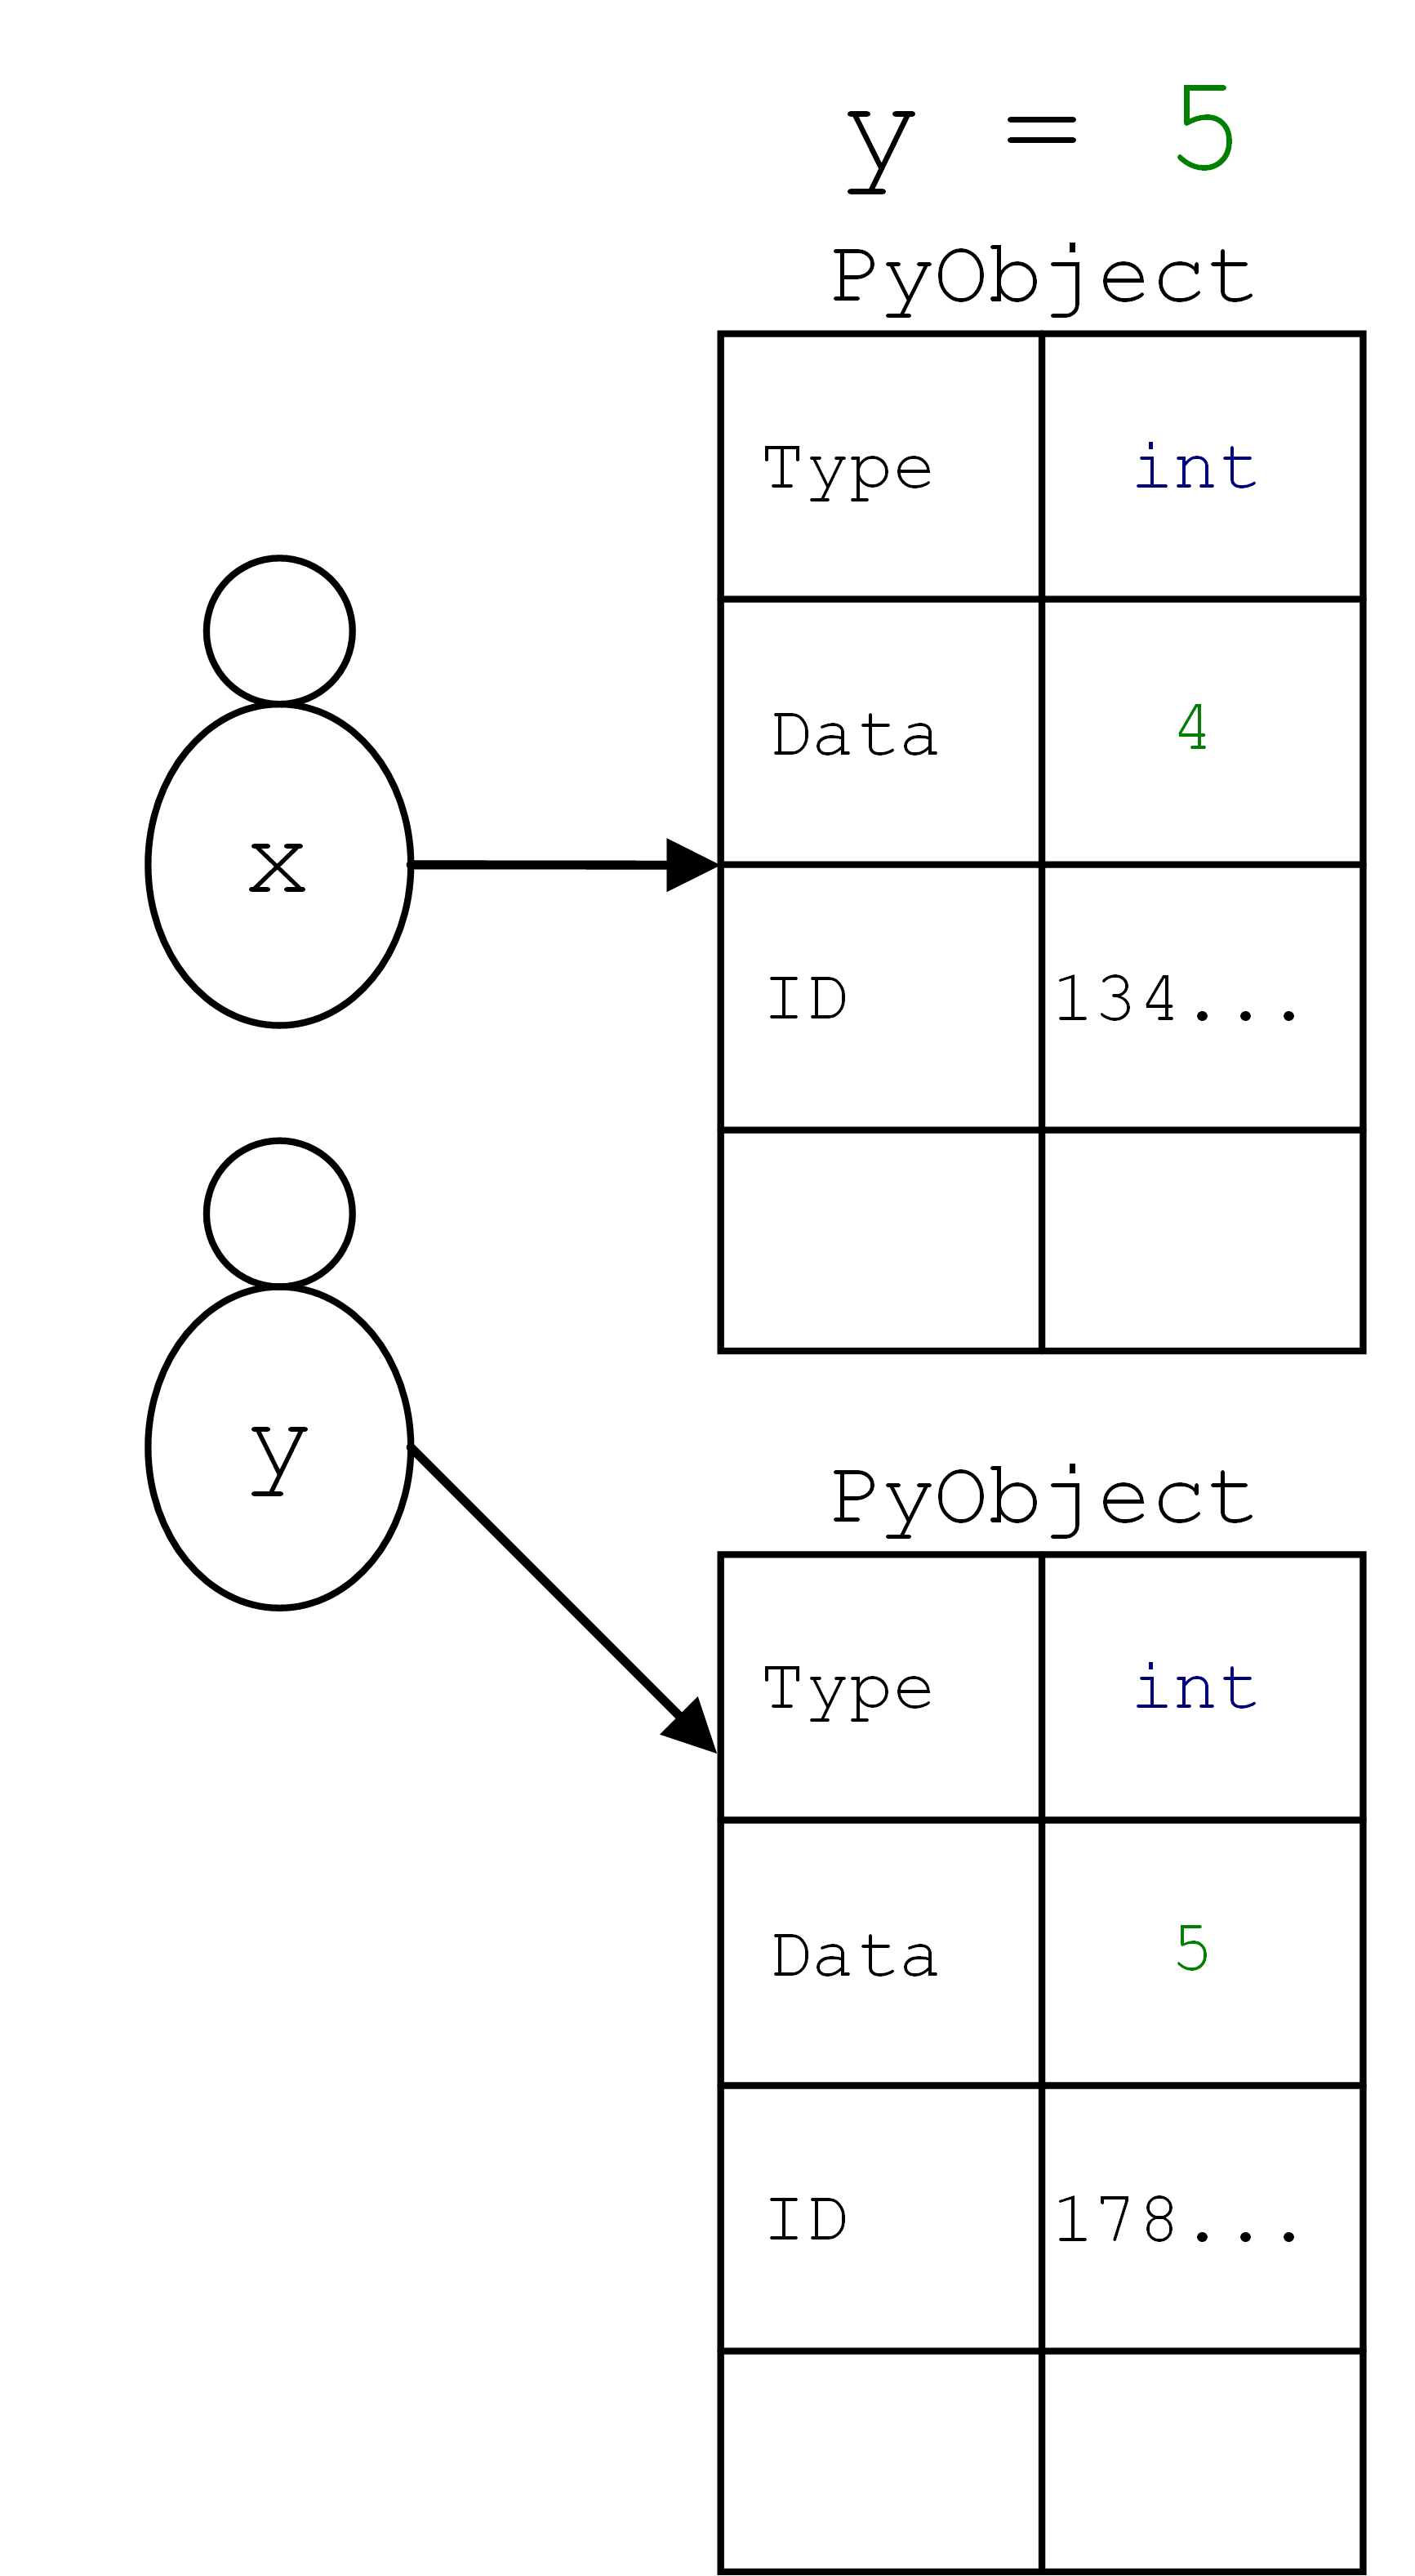
\includegraphics[width=\linewidth]{images/var_3.png}
\end{minipage}

\subsection{Built-in Data Types}
\begin{center}
    \begin{tabular}{llll}
        \toprule
        \textbf{Category} & \textbf{Data Type} & \textbf{Mutability} & \textbf{False Value} \\ \midrule
        \textbf{None} & \texttt{NoneType} & Immutable & \texttt{None} \\ \addlinespace
        \textbf{Numeric} & \texttt{int} & Immutable & \texttt{0} \\
        & \texttt{float} & Immutable & \texttt{0.0} \\
        & \texttt{bool} & Immutable & \texttt{False} \\
        & \texttt{complex} & Immutable & \texttt{0 + 0j} \\ \addlinespace
        \textbf{Sequence} & \texttt{str} & Immutable & \texttt{''} \\
        & \texttt{list} & Mutable & \texttt{[]} \\
        & \texttt{tuple} & Immutable & \texttt{()} \\
        & \texttt{bytes} & Immutable & \texttt{b''} \\
        & \texttt{bytearray} & Mutable & \texttt{bytearray(b'')} \\ \addlinespace
        \textbf{Sets} & \texttt{set} & Mutable & \texttt{set()} \\
        & \texttt{frozenset} & Immutable & \texttt{frozenset()} \\ \addlinespace
        \textbf{Associative} & \texttt{dict} & Mutable & \texttt{\{\}} \\ \bottomrule
    \end{tabular}
\end{center}

\subsection{Mutability}
\begin{itemize}
    \item \textbf{Immutable:} Objects that cannot be modified after creation (e.g., \texttt{int}, \texttt{float}, \texttt{str}, \texttt{tuple}). Changing the value of an immutable variable actually creates a new object in memory.
    \item \textbf{Mutable:} Objects that can be modified in-place (e.g., \texttt{list}, \texttt{set}, \texttt{dict}).
\end{itemize}\vspace{1em}
The memory address of an object, can be visuasalized using the \texttt{id()} function. 

It returns a unique integer for the given object.

\section{Namespaces and Scope}
A namespace is a system (implemented as a dictionary) that ensures all names in a program are unique and can be used without conflict.

\begin{itemize}
    \item \textbf{Built-in:} Contains all integrated symbols available in Python (e.g., \texttt{print()}).
    \item \textbf{Global:} Symbols defined at the top level of a module or script.
    \item \textbf{Local:} Created for specific scopes, such as within a function.
    \item \textbf{LEGB Rule:} Python searches for names from the inside out: \textbf{L}ocal $\rightarrow$ \textbf{G}lobal $\rightarrow$ \textbf{B}uilt-in.
\end{itemize}

Built-in symbols can be overwritten by the user, however, it is not recommended.

\section{Arithmetic and Magic Methods}
\begin{itemize}
    \item \textbf{Special Operators:} \texttt{//} (integer division), \texttt{\%} (modulo/remainder), and \texttt{**} (exponentiation).
    \item \textbf{Syntactic Sugar:} Operators are just a "friendly" way to call internal methods. For example, \texttt{x + y} is internally executed as \texttt{x.\_\_add\_\_(y)}.
\end{itemize}

\begin{center}
    \small
    \begin{tabular}{lll}
    \toprule
    \textbf{Operator} & \textbf{Dunder Method} & \textbf{Description} \\ \midrule
    \texttt{x + y} & \texttt{x.\_\_add\_\_(y)} & Sum \\
    \texttt{x - y} & \texttt{x.\_\_sub\_\_(y)} & Difference \\
    \texttt{x * y} & \texttt{x.\_\_mul\_\_(y)} & Product \\
    \texttt{x / y} & \texttt{x.\_\_truediv\_\_(y)} & Quotient \\
    \texttt{x // y} & \texttt{x.\_\_floordiv\_\_(y)} & Floored quotient$^1$ \\
    \texttt{x \% y} & \texttt{x.\_\_mod\_\_(y)} & Remainder (Modulo)$^1$ \\
    \texttt{x ** y} & \texttt{x.\_\_pow\_\_(y)} & Exponentiation ($x^y$) \\
    \texttt{abs(x)} & \texttt{x.\_\_abs\_\_()} & Absolute value \\
    \texttt{-x} & \texttt{x.\_\_neg\_\_()} & Negative sign \\ \midrule
    \multicolumn{3}{l}{\small $^1$ Operator not defined for the data type \texttt{complex}} \\ \bottomrule
    \end{tabular}
\end{center}

\subsection*{Code Example}
Ecco come Python interpreta gli operatori dietro le quinte:

\begin{lstlisting}[language=Python]
# Standard operator usage
result_a = 5 + 5

# Behind the scenes (Magic Method)
result_b = (5).__add__(5)

print(result_a == result_b) # Output: True
\end{lstlisting}